\documentclass[aspectratio=169,11pt]{beamer}

\usepackage{iftex}
\ifXeTeX
  \usepackage{fontspec}
  \IfFontExistsTF{DejaVu Serif}{
    \setmainfont{DejaVu Serif}
  }{
    \setmainfont{Latin Modern Roman}
  }
  \IfFontExistsTF{DejaVu Sans}{
    \setsansfont{DejaVu Sans}
  }{}
  \IfFontExistsTF{DejaVu Sans Mono}{
    \setmonofont{DejaVu Sans Mono}
  }{}
\fi
\usepackage{amsmath}
\usepackage{amssymb}
\usepackage{array}
\usepackage{booktabs}
\usepackage{graphicx}
\usepackage{siunitx}
\usepackage{xcolor}
\usepackage{xurl}

\usetheme{Madrid}
\usecolortheme{default}
\setbeamertemplate{navigation symbols}{}
\setbeamertemplate{footline}[frame number]
\graphicspath{{../images/baseline_comparison_20260509/}{../images/lono_20260509/}{images/baseline_comparison_20260509/}{images/lono_20260509/}}
\urlstyle{same}

\definecolor{aaltoBlue}{RGB}{0,83,155}
\definecolor{goodGreen}{RGB}{35,120,75}
\definecolor{warnRed}{RGB}{170,55,55}
\definecolor{softGray}{RGB}{245,246,248}

\newcommand{\good}[1]{\textcolor{goodGreen}{#1}}
\newcommand{\warn}[1]{\textcolor{warnRed}{#1}}
\newcommand{\blue}[1]{\textcolor{aaltoBlue}{#1}}
\newcommand{\sourcepath}[1]{{\scriptsize\url{#1}}}
\newcommand{\sourcenote}[1]{\vfill{\tiny\textcolor{gray!70!black}{Source: \url{#1}}}}
\newcolumntype{L}[1]{>{\raggedright\arraybackslash}p{#1}}
\newcolumntype{R}[1]{>{\raggedleft\arraybackslash}p{#1}}

\title[Baseline Comparison]{Baseline Comparison and \texorpdfstring{\(\Delta P^{0.5}\)}{Delta P exponent 0.5} Stage-3 MLP}
\subtitle{Hiroyasu--Arai, Naber--Siebers, Sparse GP, and five-seed external clean evaluation}
\author{Linan Jiang}
\institute{Aalto University}
\date{9 May 2026}

\begin{document}

\begin{frame}
  \titlepage
  \vspace{-0.8em}
  \centering
  \tiny Frozen slide data snapshot:
  \url{Thesis/generated/baseline_comparison_20260509/}
\end{frame}

\begin{frame}{Evidence Chain for This Deck}
\small
\begin{tabular}{L{0.24\linewidth}L{0.33\linewidth}L{0.34\linewidth}}
\toprule
Question & Method & How to read it \\
\midrule
Can a physics formula explain the data? &
Hiroyasu--Arai and Naber--Siebers &
Deterministic physics correlations; strong but rigid references. \\
Is a standard ML baseline already enough? &
Sparse heteroscedastic GP &
Non-parametric and uncertainty-aware; checks whether the MLP is just benefiting from small-data luck. \\
Is the neural network stable? &
\(\Delta P^{0.5}\) Stage-3, 5 seeds &
Looks at seed-to-seed variation instead of a single-run headline. \\
Does it generalize to unseen nozzles? &
Leave-one-nozzle-out &
Removes an entire nozzle family from training to test true OOD interpolation/extrapolation pressure. \\
Is the uncertainty trustworthy? &
Coverage, reliability, CRPS, PIT &
Separates "small error" from "statistically meaningful error bars." \\
\bottomrule
\end{tabular}

\vspace{0.5em}
\footnotesize
The point of this deck is not to report only one RMSE number. It explains accuracy, tail error, calibration,
seed stability, and OOD behaviour inside one evaluation protocol.
\end{frame}

\begin{frame}{Metric Meaning: Accuracy, Tail, and Calibration}
\small
\begin{columns}[T,onlytextwidth]
\begin{column}{0.48\linewidth}
\begin{block}{Point-prediction error}
\footnotesize
\[
\mathrm{RMSE}=\sqrt{\frac{1}{n}\sum_i(\hat y_i-y_i)^2},
\quad
\mathrm{MAE}=\frac{1}{n}\sum_i|\hat y_i-y_i|.
\]
RMSE is more sensitive to large errors; MAE is closer to the everyday meaning of average millimetre error.
\[
\mathrm{Bias}=\frac{1}{n}\sum_i(\hat y_i-y_i)
\]
is used to detect systematic over- or under-prediction.
\end{block}
\end{column}

\begin{column}{0.48\linewidth}
\begin{block}{Tail error and uncertainty}
\footnotesize
\[
P95=\mathrm{quantile}_{0.95}(|\hat y-y|)
\]
means that 95\% of the pointwise errors fall below this value, which directly reflects worst-case tail behaviour.
\[
\mathrm{Coverage}_{k\sigma}
=\Pr(|y-\mu|\leq k\sigma).
\]
If Gaussian predictions are well calibrated, 1\(\sigma\)/2\(\sigma\) should be close to
0.683/0.954. Values above nominal indicate over-coverage, which is usually conservative but less sharp.
\end{block}
\end{column}
\end{columns}
\end{frame}

\begin{frame}{Protocol Meaning: In-Pipeline vs External Clean}
\small
\begin{block}{In-pipeline 5-seed bootstrap}
\footnotesize
Each seed re-runs the full Stage-1/2/3 pipeline, and the winner metrics are computed on that seed's post-evaluation
test subset. The bootstrap object is the seed-level metric: the five seeds are resampled with replacement to produce
an empirical distribution of the mean and a 95\% interval.
It answers: \textbf{does training randomness change the conclusion?}
\end{block}

\begin{block}{External clean protocol}
\footnotesize
The trained models are then evaluated on one shared full-clean diagnostic set:
\num{795561} points, \num{33845} trajectories. It answers:
\textbf{which method is more accurate on the same large external clean set?}
\end{block}

\begin{block}{Strict wording}
\footnotesize
These two protocols cannot be merged into a single number without care. This deck uses the in-pipeline result for seed
stability and the external clean result for the headline model comparison.
\end{block}
\end{frame}

\begin{frame}{One-Sentence Conclusion}
\small
\begin{block}{Under the same external clean evaluation protocol}
The five-seed mean of the Stage-3 MLP with \(\Delta P^{0.5}\) feature engineering reaches
\good{RMSE \SI{6.211}{mm} \(\pm\) \SI{0.283}{mm}}
on \num{795561} points and \num{33845} trajectories.
\end{block}

\vspace{0.4em}
\begin{columns}[T,onlytextwidth]
\begin{column}{0.48\linewidth}
\begin{block}{Against physical baselines}
\begin{itemize}
  \item vs Hiroyasu--Arai: RMSE \good{-37.7\%}, MAE \good{-40.3\%}.
  \item vs Naber--Siebers: RMSE \good{-29.7\%}, MAE \good{-32.3\%}.
  \item vs sparse GP: RMSE \good{-10.0\%}, MAE \good{-11.9\%}.
\end{itemize}
\end{block}
\end{column}

\begin{column}{0.48\linewidth}
\begin{block}{Against the older MLP}
\begin{itemize}
  \item Old \(\Delta P^{0.25}\), seed 42: RMSE \SI{6.696}{mm}.
  \item New \(\Delta P^{0.5}\), five-seed mean: RMSE \SI{6.211}{mm}.
  \item Sparse GP mean: RMSE \SI{6.898}{mm}, MAE \SI{5.206}{mm}.
\end{itemize}
\end{block}
\end{column}
\end{columns}

\sourcenote{snapshot/analysis_summary.md}
\end{frame}

\begin{frame}{Headline Comparison Table}
\scriptsize
{\setlength{\tabcolsep}{3pt}
\begin{tabular}{L{0.34\linewidth}R{0.09\linewidth}R{0.09\linewidth}R{0.09\linewidth}R{0.09\linewidth}R{0.09\linewidth}R{0.09\linewidth}}
\toprule
Model & RMSE & MAE & Bias & P95 & 1\(\sigma\) cov. & 2\(\sigma\) cov. \\
\midrule
Hiroyasu--Arai calibrated & 9.974 & 7.686 & +0.625 & 20.493 & 0.536 & 0.886 \\
Naber--Siebers delay & 8.840 & 6.780 & -0.344 & 17.922 & 0.620 & 0.893 \\
Stage-3 MLP \(\Delta P^{0.25}\), seed 42 & 6.696 & 4.875 & -1.149 & 14.118 & 0.745 & 0.979 \\
\good{Stage-3 MLP \(\Delta P^{0.5}\), 5-seed mean} & \good{6.211} & \good{4.587} & \good{-0.838} & \good{13.029} & \good{0.774} & \good{0.981} \\
Sparse heteroscedastic GP, 5-seed mean & 6.898 & 5.206 & -1.184 & 14.365 & 0.670 & 0.950 \\
\bottomrule
\end{tabular}
}

\vspace{0.7em}
\small
\begin{block}{How to position this in the thesis}
The older MLP result should no longer be treated as the neural-network headline. It is now only a reference row
before the \(\Delta P\) exponent was changed from 0.25 to 0.5. The GP is a strong ML baseline: its calibration is
close to nominal, but its accuracy is still below the new MLP five-seed mean.
\end{block}

\sourcenote{snapshot/headline_comparison.csv}
\end{frame}

\begin{frame}{Physical Baseline I: Hiroyasu--Arai / Zhou}
\small
\begin{block}{Theory role}
\footnotesize
Hiroyasu--Arai writes spray penetration as a staged empirical law: the early phase is controlled by injection
velocity, and after breakup it transitions to an entrainment-dominated square-root time scaling. The Zhou-style
post-injection extension adds a \((t-t_i)^{1/4}\) branch after EOI.
\end{block}

\vspace{-0.2em}
\[
S(t)=
\begin{cases}
k_v\sqrt{2\Delta P/\rho_l}\,t, & t<t_b,\\[0.25em]
k_p(\Delta P/\rho_a)^{1/4}d_n^{1/2}t^{1/2}, & t\ge t_b.
\end{cases}
\]
\[
t_b=k_{bt}\frac{\rho_l d_n}{\sqrt{\rho_a\Delta P}},
\qquad
S_{\mathrm{post}}\propto
(\Delta P/\rho_a)^{1/4}d_n^{1/2}t_i^{1/4}(t-t_i)^{1/4}.
\]

\footnotesize
This study uses the calibrated version as the strong physics baseline; its uncertainty comes from residual statistics,
not from an input-dependent learned \(\sigma(x,t)\).
\end{frame}

\begin{frame}{Physical Baseline II: Naber--Siebers}
\small
\begin{block}{Theory role}
\footnotesize
Naber--Siebers is a mixing-limited penetration correlation. It folds the main operating-condition dependence into
the physical scale \(A\), then multiplies by a \(\sqrt{t}\)-type time growth.
\end{block}

\[
S(t)=K\,
\underbrace{\left(\frac{\Delta P}{\rho_a}\right)^{1/4}d_n^{1/2}}_{A_{\mathrm{NS}}}
\sqrt{\max(t-t_d,0)}.
\]

\begin{itemize}
  \item \(K\): global scale; \(t_d\): hydraulic/observation delay.
  \item Optional cone-angle variant can use video-measured \(\theta\), but the headline comparison uses the delay
  variant, which does not require an oracle visual feature.
  \item The point is to give the MLP an interpretable, low-degree-of-freedom, physically rigid baseline.
\end{itemize}
\end{frame}

\begin{frame}{GP Learning Target: Swapping the Prior for MLP Regression}
\small
\begin{block}{First write the problem as the same supervised-learning task as the MLP}
\footnotesize
Each sample is
\[
x_i=[t,\;\mathrm{tilt},\;\mathrm{plumes},\;t_{\mathrm{inj}},\;p_{\mathrm{ctrl}}]_i,
\qquad
z_i=\frac{S_i}{A_i}.
\]
where
\[
A_i=(\Delta P_i)^{0.5}\rho_{a,i}^{-0.25}d_{n,i}^{0.5}.
\]
The MLP learns \(x\mapsto z\). The GP baseline learns the same target and is then multiplied by \(A_i\) to return
to millimetres.
\end{block}

\begin{block}{The difference is only the function assumption}
\footnotesize
MLP: represent the function explicitly with parameters, \(z_\theta(x)\).\\
GP: do not write a fixed network first; instead place a probabilistic prior directly over the function \(f(x)\):
\[
z_i=f(x_i)+\epsilon_i.
\]
\end{block}
\end{frame}

\begin{frame}{GP Definition: Not a Curve, but a Family of Joint Gaussians}
\small
\begin{block}{Finite-dimensional definition}
\footnotesize
If, for any finite input set \(X=[x_1,\ldots,x_n]\), the function values satisfy
\[
\mathbf f_X=[f(x_1),\ldots,f(x_n)]^\top
\sim
\mathcal N(\mathbf m_X,K_{XX}),
\]
then
\[
f(x)\sim\mathcal{GP}(m(x),k(x,x')).
\]
\end{block}

\begin{columns}[T,onlytextwidth]
\begin{column}{0.48\linewidth}
\begin{block}{Mean function}
\footnotesize
\[
(\mathbf m_X)_i=m(x_i)
\]
This implementation uses a constant mean so that the data learn the global offset.
\end{block}
\end{column}
\begin{column}{0.48\linewidth}
\begin{block}{Kernel / covariance}
\footnotesize
\[
(K_{XX})_{ij}=k(x_i,x_j)
\]
The kernel determines how similar the function values at two input points should be.
\end{block}
\end{column}
\end{columns}
\end{frame}

\begin{frame}{Kernel Used Here: ARD Mat\'ern-\(5/2\)}
\small
\begin{block}{Distance is scaled by learned length-scales}
\footnotesize
\[
r^2(x,x')=\sum_{j=1}^{5}\left(\frac{x_j-x'_j}{\ell_j}\right)^2.
\]
\(\ell_j\) is the length-scale for feature dimension \(j\). A large \(\ell_j\) means the function is insensitive to
that feature; a small \(\ell_j\) means even small changes in that feature can move the prediction.
\end{block}

\begin{block}{Mat\'ern-\(5/2\) covariance}
\footnotesize
\[
k_\theta(x,x')=\sigma_f^2
\left(1+\sqrt{5}r+\frac{5r^2}{3}\right)\exp(-\sqrt{5}r).
\]
It is smoother than a rough kernel, but less overly smooth than an RBF kernel, which suits spray-penetration
functions with transient behaviour.
\end{block}

\vspace{-0.2em}
\footnotesize
Code mapping: \texttt{ScaleKernel(MaternKernel(nu=2.5, ard\_num\_dims=5))}.
\end{frame}

\begin{frame}{Exact GP Derivation: Joint Gaussian over Train and Test Points}
\small
\begin{block}{Homoscedastic observation noise, starting from the simplest case}
\footnotesize
\[
\mathbf z=\mathbf f_X+\boldsymbol\epsilon,
\qquad
\boldsymbol\epsilon\sim\mathcal N(0,\sigma_n^2I).
\]
For test inputs \(X_*\), the joint distribution is
\[
\begin{bmatrix}
\mathbf z\\
\mathbf f_*
\end{bmatrix}
\sim
\mathcal N\left(
\begin{bmatrix}
\mathbf m_X\\
\mathbf m_*
\end{bmatrix},
\begin{bmatrix}
K_{XX}+\sigma_n^2I & K_{X*}\\
K_{*X} & K_{**}
\end{bmatrix}
\right).
\]
\end{block}

\begin{block}{The conditional Gaussian formula is the GP prediction formula}
\footnotesize
\[
\mu_*=\mathbf m_*+K_{*X}(K_{XX}+\sigma_n^2I)^{-1}(\mathbf z-\mathbf m_X),
\]
\[
\Sigma_*=K_{**}-K_{*X}(K_{XX}+\sigma_n^2I)^{-1}K_{X*}.
\]
These two lines are just "weighted averaging from similar training points, plus uncertainty."
\end{block}
\end{frame}

\begin{frame}{Why Not Use an Exact GP Directly on This Dataset?}
\small
\begin{block}{Hyperparameter learning comes from the marginal likelihood}
\footnotesize
Let \(K_y=K_{XX}+\sigma_n^2I\). Then
\[
\log p(\mathbf z|X,\theta)
=-\frac{1}{2}(\mathbf z-\mathbf m)^\top K_y^{-1}(\mathbf z-\mathbf m)
-\frac{1}{2}\log|K_y|-\frac{n}{2}\log 2\pi.
\]
The first term rewards fit, the second penalizes an overly complex covariance, and the third is constant.
\end{block}

\begin{block}{The bottleneck}
\footnotesize
To compute \(K_y^{-1}\mathbf z\) and \(\log|K_y|\), one usually needs a Cholesky factorization:
\[
K_y=LL^\top,\qquad \mathrm{cost}=O(n^3),\quad \mathrm{memory}=O(n^2).
\]
Here each trajectory expands into many time points, and the number of training points per seed can reach the million
range. So an exact GP is infeasible and we need a sparse variational GP.
\end{block}
\end{frame}

\begin{frame}{Sparse GP: Compressing Function Information with Inducing Points}
\small
\begin{block}{Core idea}
\footnotesize
Choose \(m\ll n\) inducing inputs
\[
Z=[z_1^{(u)},\ldots,z_m^{(u)}],
\qquad
\mathbf u=f(Z).
\]
They are not training labels, but support points of the function. Training learns the function distribution around
these points and then uses them to explain all \(n\) training samples.
\end{block}

\begin{block}{Conditional structure}
\footnotesize
The GP prior gives
\[
p(\mathbf f,\mathbf u)=p(\mathbf f|\mathbf u)p(\mathbf u),
\qquad
p(\mathbf u)=\mathcal N(\mathbf m_Z,K_{ZZ}).
\]
If \(m=256\), the main matrix operations shift from \(n\times n\) to \(m\times m\) and minibatch covariance terms.
\end{block}

\footnotesize
This implementation initializes 256 inducing points with K-means over the training inputs and allows their positions
to keep learning.
\end{frame}

\begin{frame}{Variational GP: Replacing the Posterior \(p(u|D)\) with Optimizable \(q(u)\)}
\small
\begin{block}{Variational distribution}
\footnotesize
The exact posterior \(p(\mathbf u|\mathcal D)\) is hard to compute directly, so we set
\[
q(\mathbf u)=\mathcal N(\mathbf m_u,S_u),
\]
where \(\mathbf m_u\) and \(S_u\) are trainable parameters. For any training-point function values:
\[
q(\mathbf f)=\int p(\mathbf f|\mathbf u)q(\mathbf u)\,d\mathbf u.
\]
\end{block}

\begin{block}{ELBO: optimize a computable lower bound}
\footnotesize
\[
\mathcal L
=
\sum_{i=1}^{n}
\mathbb E_{q(f_i)}[\log p(z_i|f_i)]
-\mathrm{KL}\!\left(q(\mathbf u)\,\|\,p(\mathbf u)\right).
\]
The first term demands that the predictions explain the data; the second prevents \(q(u)\) from drifting too far
from the GP prior. In minibatch training, the batch likelihood term is scaled by \(n/|\mathcal B|\).
\end{block}
\end{frame}

\begin{frame}{The Heteroscedastic GP in This Thesis: Two SVGPs in Series}
\small
\begin{block}{Stage 1: mean SVGP}
\footnotesize
\[
f_\mu(x)\sim\mathcal{GP}(m_\mu,k_\mu),
\qquad
z_i=f_\mu(x_i)+\epsilon_i.
\]
After training we get
\[
\hat\mu_z(x)=\mathbb E[f_\mu(x)].
\]
\end{block}

\begin{block}{Stage 2: log-variance SVGP}
\footnotesize
First use the mean GP to compute residuals on the training set:
\[
r_i=z_i-\hat\mu_z(x_i).
\]
Then build a variance target:
\[
g_i=\log(r_i^2+\varepsilon).
\]
The second SVGP learns
\[
f_v(x)\approx g,\qquad
\hat\sigma_z^2(x)=\exp(\hat f_v(x)+b).
\]
\(b\) is a log-variance bias correction fitted on validation data.
\end{block}
\end{frame}

\begin{frame}{From Scaled GP Output Back to Millimetre Penetration}
\small
\begin{block}{Scaled space}
\footnotesize
GP training and prediction both happen in
\[
z=\frac{S}{A_{\mathrm{scale}}}
\]
space, so the outputs are
\[
\hat\mu_z(x),\qquad \hat\sigma_z(x).
\]
\end{block}

\begin{block}{Physical space}
\footnotesize
Back in penetration units:
\[
\hat\mu_S(x)=A_{\mathrm{scale}}(x)\hat\mu_z(x),
\qquad
\hat\sigma_S(x)=A_{\mathrm{scale}}(x)\hat\sigma_z(x).
\]
RMSE, MAE, P95, and coverage are all computed using \(\hat\mu_S,\hat\sigma_S\) and the true \(S\) in millimetres.
\end{block}

\begin{block}{One implementation detail}
\footnotesize
The headline GP uses residual log-variance as the main uncertainty source;
\texttt{include\_mean\_posterior\_var=false}, meaning we do not add the mean GP posterior variance to \(\sigma\).
\end{block}
\end{frame}

\begin{frame}{Mapping the Formulas to Project Code}
\scriptsize
\begin{tabular}{L{0.26\linewidth}L{0.34\linewidth}L{0.31\linewidth}}
\toprule
Mathematical object & Implementation & Interpretation \\
\midrule
\(x\) &
\texttt{a\_only} features &
time, tilt, plume count, injection duration, control backpressure. \\
\(z=S/A\) &
\texttt{target\_scaled} &
The same \(\Delta P^{0.5}\) scale used by the Stage-3 MLP. \\
\(k_\theta\) &
ARD Mat\'ern-\(5/2\) &
One length-scale per feature dimension. \\
\(Z,\mathbf u\) &
256 inducing points &
K-means initialization, with trainable positions. \\
\(q(u)\) &
Cholesky variational distribution &
GPyTorch sparse variational posterior. \\
\(\mathcal L\) &
\texttt{VariationalELBO} &
Minibatch Adam, mean and logvar each trained for up to 80 epochs. \\
\(\sigma(x)\) &
Second SVGP on \(\log r^2\) &
Two-stage heteroscedastic uncertainty. \\
\bottomrule
\end{tabular}

\vspace{0.5em}
\footnotesize
Code entry point: \sourcepath{MLP/MLP_training/run_gp_baseline.py}
\end{frame}

\begin{frame}{Why Is This GP Baseline Fair, Yet Still Worse than the MLP?}
\small
\begin{block}{Fairness}
\footnotesize
The GP uses the same split, the same five seeds, the same \(A_{\mathrm{scale}}\) target, the same controllable
input features, and the same external clean diagnostic set as the MLP.
\end{block}

\begin{block}{GP strength}
\footnotesize
The kernel prior imposes a strong smoothness assumption, the SVGP gives probabilistic prediction, and the
two-stage log-variance model lets uncertainty vary with the input. So this is not a weak baseline; it does bring
coverage close to nominal.
\end{block}

\begin{block}{MLP strength}
\footnotesize
The Stage-3 MLP is more than a plain regressor: it inherits the full trajectory structure of the fitted target and
then refines the raw CDF in the early reliable region. The GP baseline learns the same pointwise targets but does
not have that teacher/raw two-stage training mechanism.
\end{block}
\end{frame}

\begin{frame}{Can the GP Beat the MLP?}
\small
\begin{columns}[T,onlytextwidth]
\begin{column}{0.48\linewidth}
\begin{block}{Accuracy: no}
{\setlength{\tabcolsep}{3pt}
\begin{tabular}{L{0.48\linewidth}R{0.20\linewidth}R{0.20\linewidth}}
\toprule
Metric & MLP & GP \\
\midrule
RMSE & \good{6.211} & 6.898 \\
MAE & \good{4.587} & 5.206 \\
P95 & \good{13.029} & 14.365 \\
\bottomrule
\end{tabular}
}

\vspace{0.4em}
\footnotesize
Relative to the new MLP, the GP is worse by 11.1\% / 13.5\% / 10.2\% in RMSE / MAE / P95.
\end{block}
\end{column}

\begin{column}{0.48\linewidth}
\begin{block}{Calibration: the GP is closer to nominal}
{\setlength{\tabcolsep}{3pt}
\begin{tabular}{L{0.48\linewidth}R{0.20\linewidth}R{0.20\linewidth}}
\toprule
Metric & MLP & GP \\
\midrule
1\(\sigma\) cov. & 0.774 & \good{0.670} \\
2\(\sigma\) cov. & 0.981 & \good{0.950} \\
\bottomrule
\end{tabular}
}

\vspace{0.4em}
\footnotesize
Gaussian nominal is 0.683/0.954. The GP uncertainty is closer to nominal, while the MLP is conservative on the
clean set.
\end{block}
\end{column}
\end{columns}

\vspace{0.2em}
\begin{block}{Conclusion}
The GP is a strong baseline, especially because it shows the uncertainty comparison is fair. But under the same
external clean protocol, it does not beat the \(\Delta P^{0.5}\) Stage-3 MLP.
\end{block}

\sourcenote{snapshot/headline_comparison.csv}
\end{frame}

\begin{frame}{OOD / LONO: What the Protocol Means}
\small
\begin{block}{Leave-one-nozzle-out protocol}
\footnotesize
LONO removes all samples from one nozzle family / experiment label from training and tests only on that held-out
group. It is stricter than an ordinary group-aware split because the test nozzle is completely unseen during training.
\end{block}

\begin{block}{What it answers}
\footnotesize
External clean eval mainly checks in-distribution performance; LONO checks whether the model can preserve physical
scaling and residual learning on unseen nozzle families. The statistical object here is fold-to-fold variation, not
seed-to-seed variation.
\end{block}

\begin{block}{Current 5-fold result}
\footnotesize
MLP \(\Delta P^{0.5}\): RMSE \(7.435\pm0.692\) mm; HA:
\(10.713\pm1.542\) mm; NS: \(9.784\pm2.102\) mm. Relative to HA/NS, RMSE drops by about 30.6\% / 24.0\%.
\end{block}
\end{frame}

\begin{frame}{LONO Result: RMSE for Each Held-Out Nozzle}
\centering
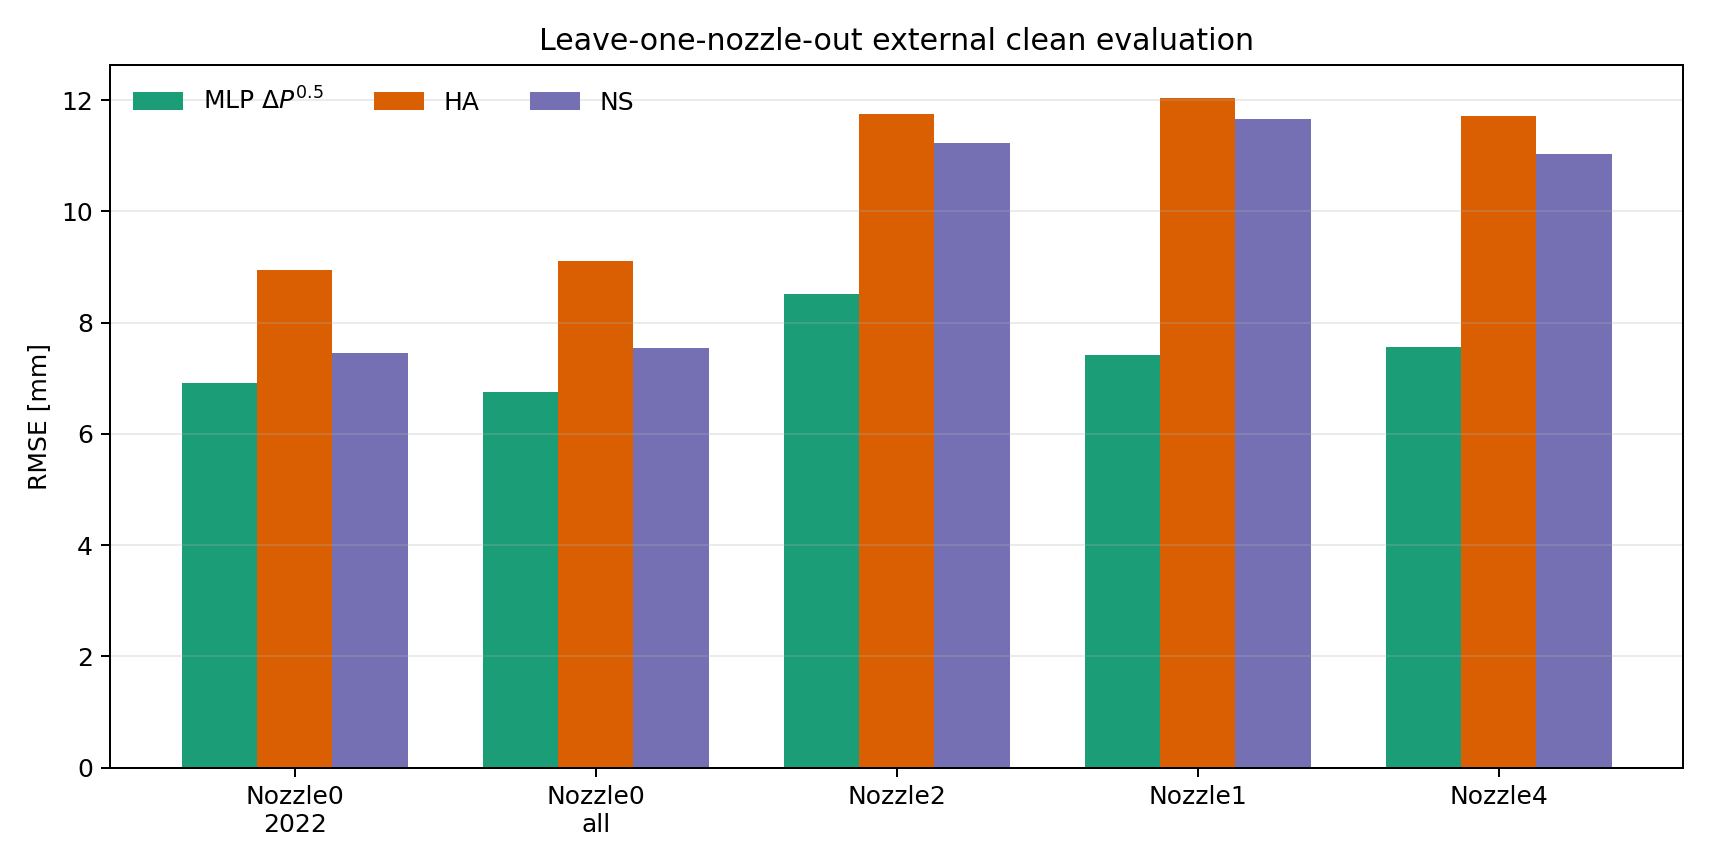
\includegraphics[width=0.92\linewidth,height=0.72\textheight,keepaspectratio]{lono_rmse_by_fold.png}

\vspace{0.15em}
\footnotesize
Across the five held-out folds, the MLP is below both HA and NS. The hardest fold is BC20241017\_HZ\_Nozzle2,
where the MLP RMSE is \SI{8.517}{mm}, still below HA \SI{11.754}{mm} and NS \SI{11.236}{mm}.

\sourcenote{MLP/runs\_mlp/lono\_pipeline\_20260509\_215613/per\_fold.csv}
\end{frame}

\begin{frame}{LONO Result: Does Coverage Collapse under OOD?}
\centering
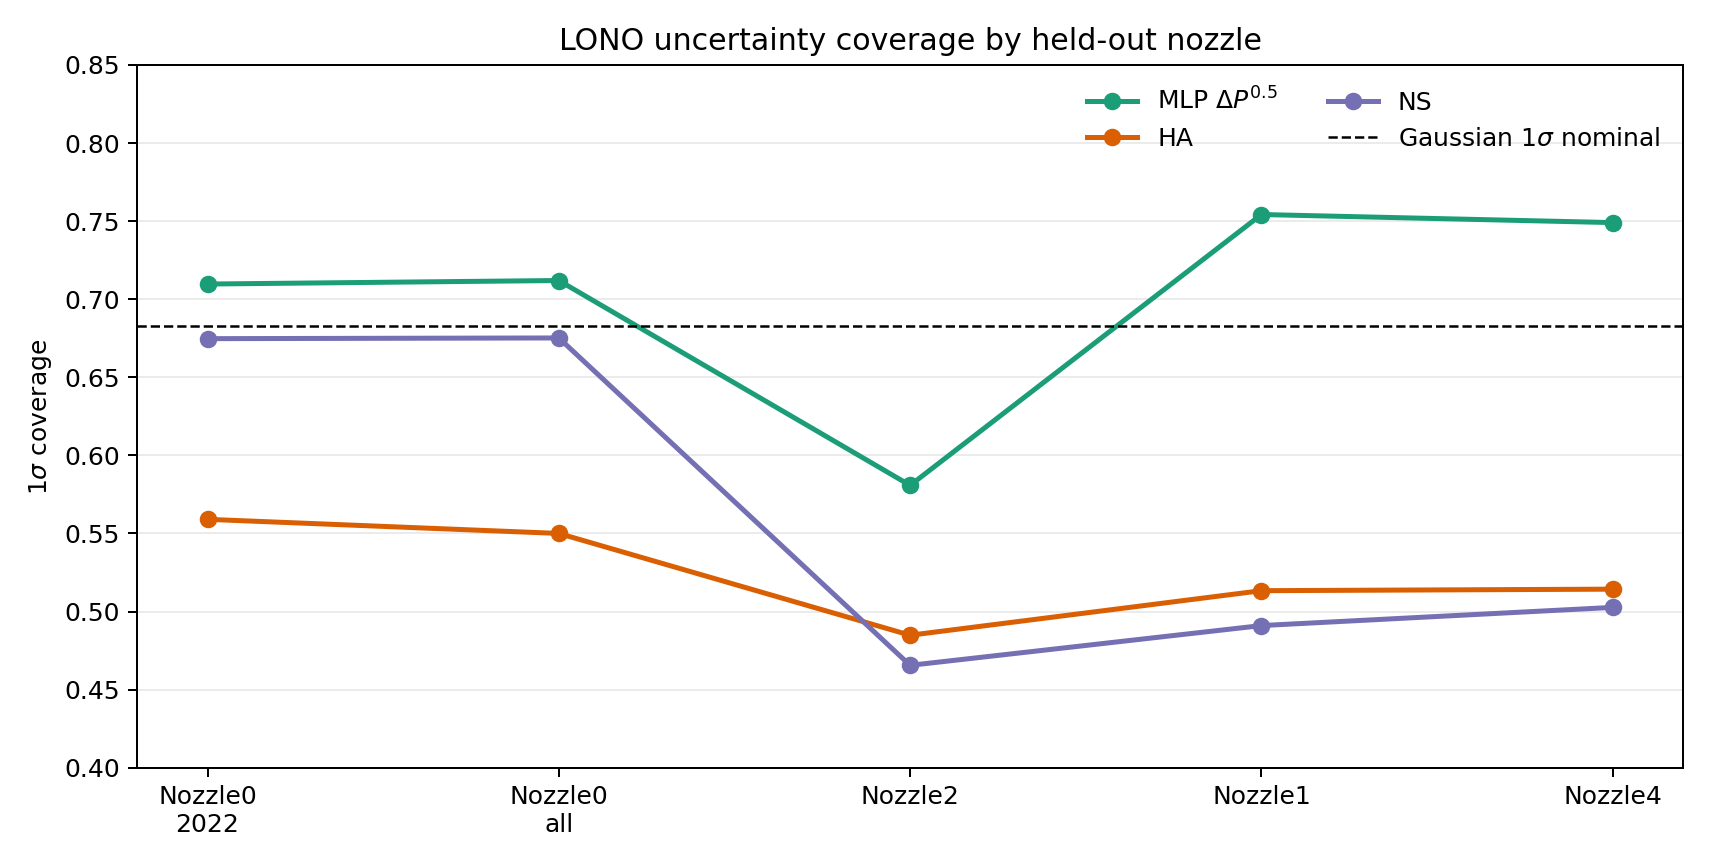
\includegraphics[width=0.92\linewidth,height=0.72\textheight,keepaspectratio]{lono_coverage_by_fold.png}

\vspace{0.15em}
\footnotesize
The MLP's mean 1\(\sigma\) coverage is 0.701, close to the Gaussian nominal 0.683. The Nozzle2 fold is clearly
under-covered, which means that nozzle family remains an OOD risk point instead of being hidden by the average.

\sourcenote{MLP/runs\_mlp/lono\_pipeline\_20260509\_215613/aggregate.csv}
\end{frame}

\begin{frame}{Error Metrics: Physical Baseline, GP, and MLP}
\centering
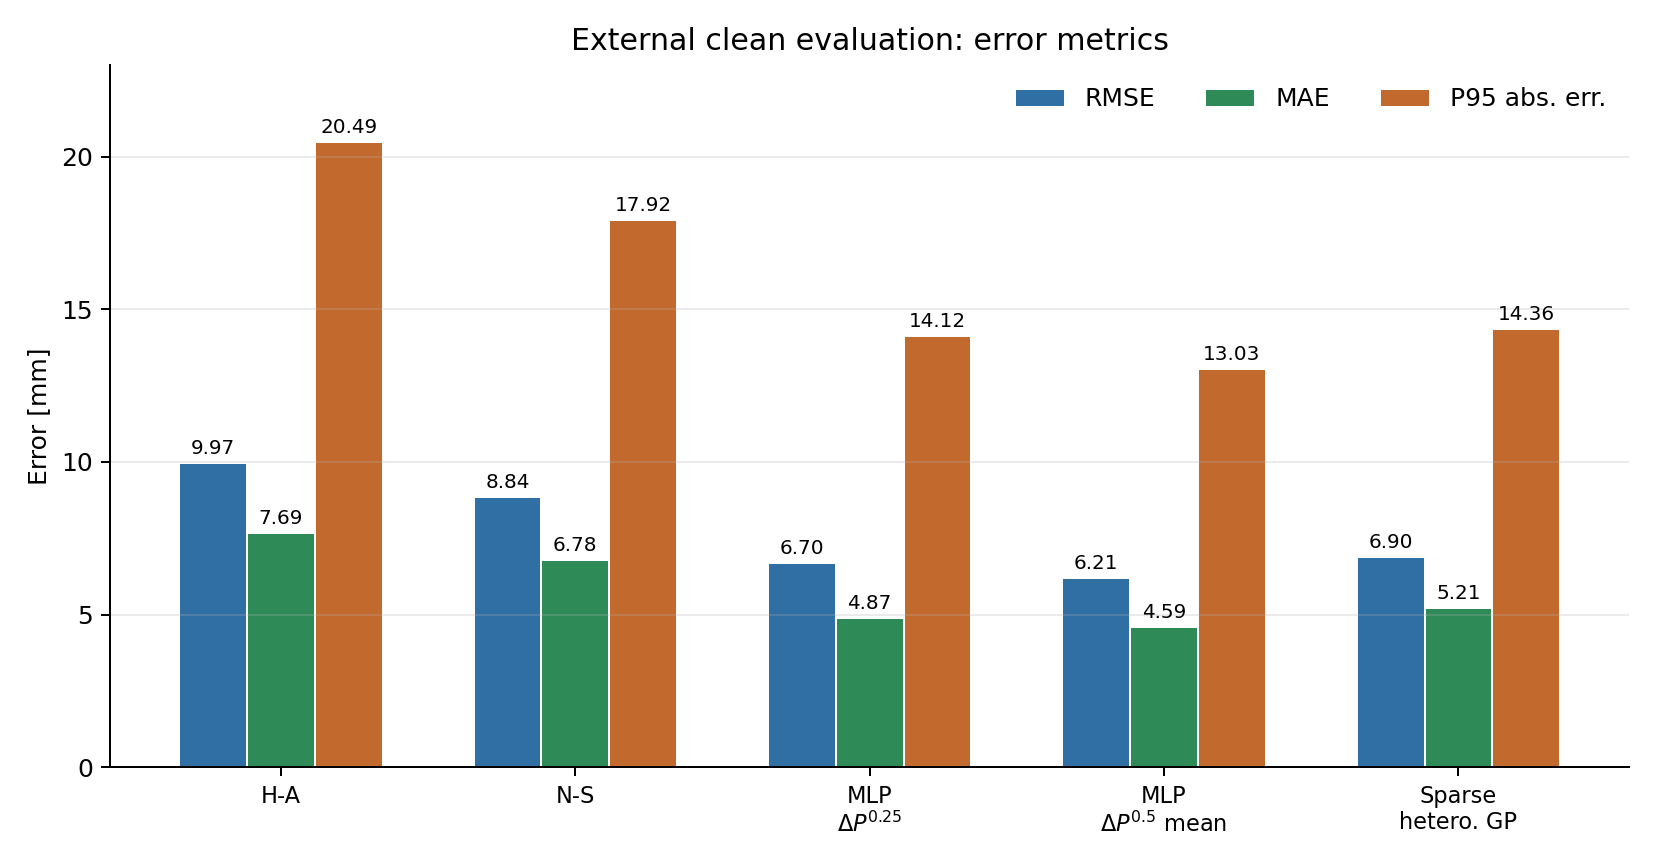
\includegraphics[width=0.90\linewidth,height=0.70\textheight,keepaspectratio]{metric_bars_rmse_mae_p95.png}

\vspace{0.2em}
\footnotesize
Under this clean evaluation protocol, the sparse GP is clearly better than the physical baselines, but it still does
not surpass the \(\Delta P^{0.5}\) Stage-3 MLP in RMSE, MAE, or tail P95 error.

\sourcenote{snapshot/headline_comparison.csv}
\end{frame}

\begin{frame}{Five-Seed External Evaluation: MLP vs GP}
\centering
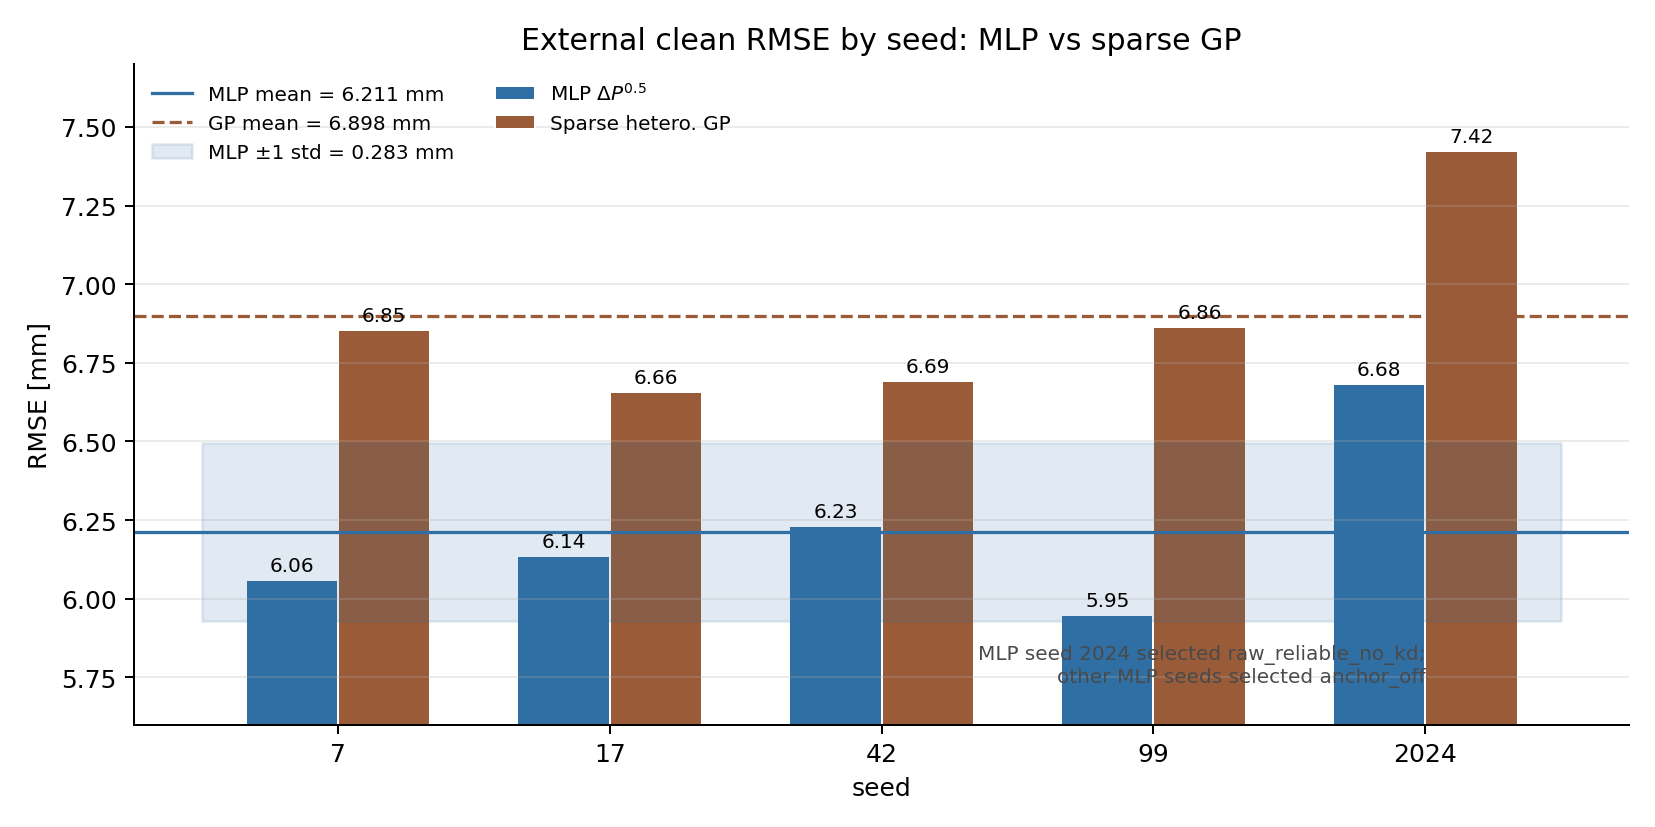
\includegraphics[width=0.92\linewidth,height=0.72\textheight,keepaspectratio]{per_seed_rmse.png}

\vspace{0.1em}
\footnotesize
The five-seed RMSE mean for the \(\Delta P^{0.5}\) MLP is \SI{6.211}{mm}; the GP five-seed external mean is
\SI{6.898}{mm}. Even the GP's best seed remains above the MLP five-seed mean.

\sourcenote{snapshot/new_mlp_5seed_aggregate.csv}
\end{frame}

\begin{frame}{Coverage: GP Is Closer to Nominal, MLP Is More Accurate}
\centering
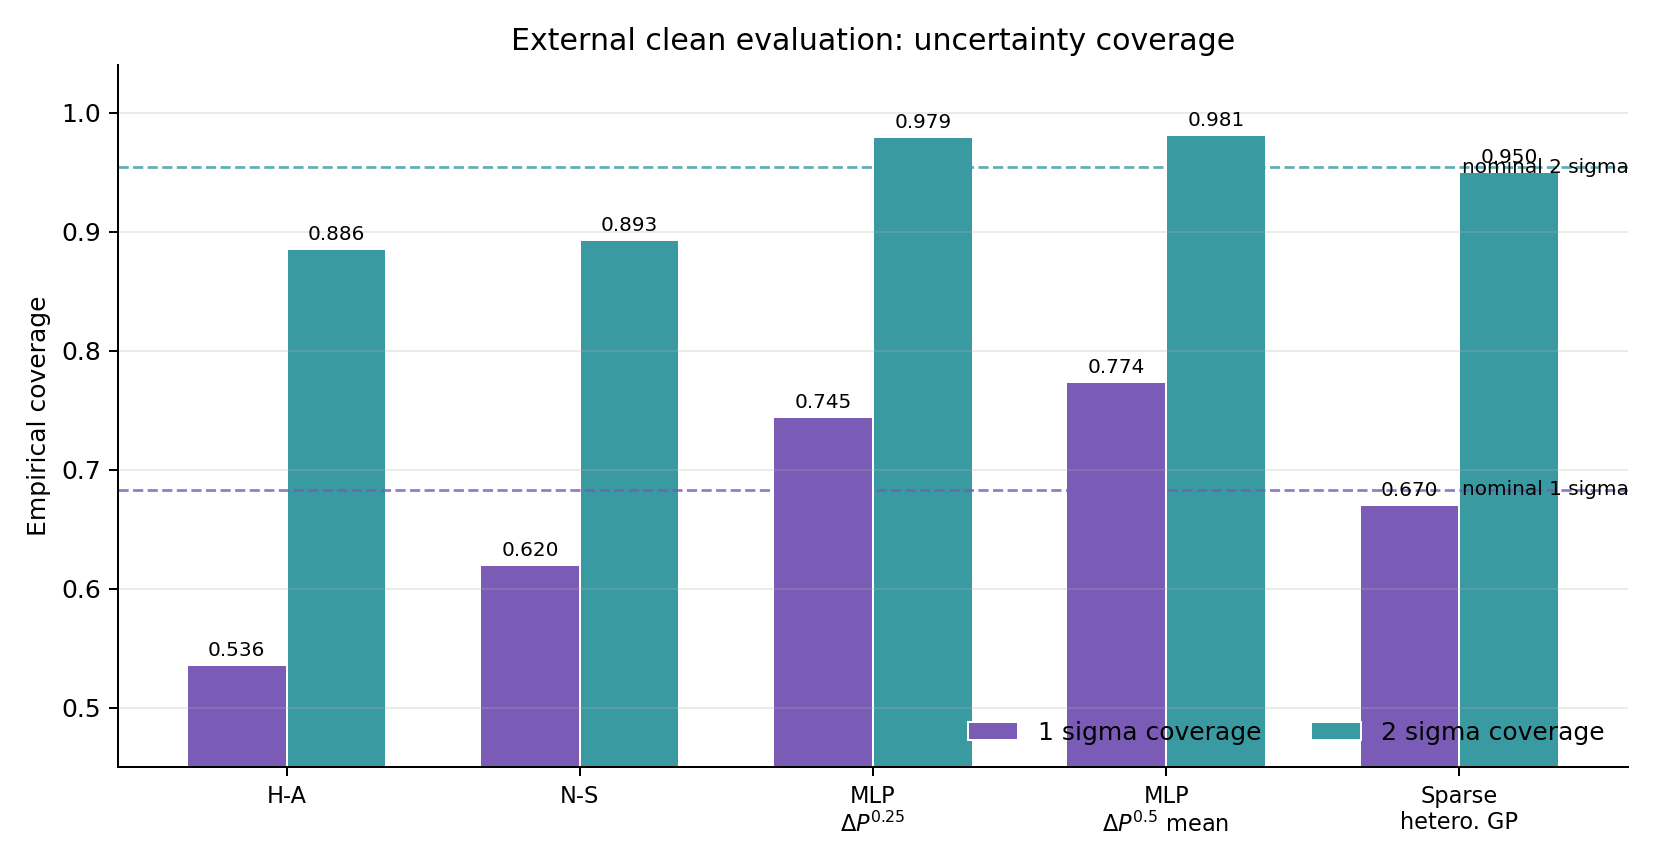
\includegraphics[width=0.90\linewidth,height=0.72\textheight,keepaspectratio]{coverage_comparison.png}

\vspace{0.1em}
\footnotesize
The new MLP has 1\(\sigma\)/2\(\sigma\) coverage of 0.774/0.981, which is over-coverage on the clean set; the GP is
0.670/0.950, closer to the Gaussian nominal 0.683/0.954. So the GP wins on calibration closeness, while the MLP wins
on accuracy.

\sourcenote{snapshot/headline_comparison.csv}
\end{frame}

\begin{frame}{Recommended Thesis Wording}
\small
\begin{block}{Abstract / introduction version}
\(\Delta P^{0.5}\) feature engineering reduced the Stage-3 MLP RMSE from
\SI{6.70}{mm} for the previous \(\Delta P^{0.25}\) seed-42 model to
\SI{6.21}{mm} \(\pm\) \SI{0.28}{mm} over five full-clean external evaluations.
\end{block}

\begin{block}{Results version}
Under the same \num{795561}-point clean diagnostic protocol, the \(\Delta P^{0.5}\) Stage-3 MLP reduced RMSE by
37.7\% relative to the calibrated Hiroyasu--Arai correlation, by 29.7\% relative to the Naber--Siebers delay model,
and by 10.0\% relative to a sparse heteroscedastic GP.
\end{block}

\sourcenote{snapshot/DATA_SOURCES.md}
\end{frame}

\begin{frame}{GP and Stability Caveat}
\small
\begin{block}{GP baseline version}
\footnotesize
The sparse heteroscedastic GP reached near-nominal uncertainty coverage (0.670/0.950 for 1\(\sigma\)/2\(\sigma\)),
but its external-clean RMSE, MAE, and P95 error were 11.1\%, 13.5\%, and 10.2\% higher than the \(\Delta P^{0.5}\)
Stage-3 MLP five-seed mean.
\end{block}

\begin{block}{Limitations version}
\footnotesize
The five-seed aggregate is a \(\Delta P^{0.5}\) Stage-3 pipeline aggregate, not a strict same-ablation seed study:
seed 2024 selected \texttt{raw\_reliable\_no\_kd}, whereas the other four seeds selected \texttt{anchor\_off}.
\end{block}

\sourcenote{snapshot/DATA_SOURCES.md}
\end{frame}

\begin{frame}{Data Sources and Refresh Entry Point}
\scriptsize
\begin{tabular}{L{0.24\linewidth}L{0.68\linewidth}}
\toprule
Item & Path \\
\midrule
Frozen snapshot &
\sourcepath{Thesis/generated/baseline_comparison_20260509/} \\
Source report &
\sourcepath{MLP/baseline/comparison_reports/gp_vs_mlp_20260509/} \\
Headline table &
\sourcepath{Thesis/generated/baseline_comparison_20260509/headline_comparison.csv} \\
Five-seed aggregate &
\sourcepath{Thesis/generated/baseline_comparison_20260509/new_mlp_5seed_aggregate.csv} \\
Per-seed eval rows &
\sourcepath{Thesis/generated/baseline_comparison_20260509/per_seed_new_mlp_eval.csv} \\
GP bootstrap &
\sourcepath{Thesis/generated/baseline_comparison_20260509/gp_bootstrap_summary.json} \\
LONO result &
\sourcepath{MLP/runs_mlp/lono_pipeline_20260509_215613/} \\
Figure builder &
\sourcepath{Thesis/generated/baseline_comparison_20260509/make_figures.py} \\
\bottomrule
\end{tabular}

\vspace{0.6em}
\begin{block}{Refresh flow}
\footnotesize
Update the comparison-report CSVs \(\rightarrow\) overwrite the CSVs in this snapshot
\(\rightarrow\) run
\sourcepath{.venv/Scripts/python.exe Thesis/generated/baseline_comparison_20260509/make_figures.py}
\(\rightarrow\) rebuild these slides.
\end{block}

\begin{block}{Protocol label}
\footnotesize
All headline rows use the external clean evaluation:
\num{795561} points, \num{33845} trajectories.
\end{block}
\end{frame}

\end{document}
